%% 
%% Copyright 2007-2020 Elsevier Ltd
%% 
%% This file is part of the 'Elsarticle Bundle'.
%% ---------------------------------------------
%% 
%% It may be distributed under the conditions of the LaTeX Project Public
%% License, either version 1.2 of this license or (at your option) any
%% later version.  The latest version of this license is in
%%    http://www.latex-project.org/lppl.txt
%% and version 1.2 or later is part of all distributions of LaTeX
%% version 1999/12/01 or later.
%% 
%% The list of all files belonging to the 'Elsarticle Bundle' is
%% given in the file `manifest.txt'.
%% 
%% Template article for Elsevier's document class `elsarticle'
%% with harvard style bibliographic references

\documentclass[preprint,12pt,authoryear]{elsarticle}
%\documentclass[10pt,final,journal,compsoc,a4paper]{IEEEtran}
%% Use the option review to obtain double line spacing
%% \documentclass[authoryear,preprint,review,12pt]{elsarticle}

%% Use the options 1p,twocolumn; 3p; 3p,twocolumn; 5p; or 5p,twocolumn
%% for a journal layout:
%% \documentclass[final,1p,times,authoryear]{elsarticle}
%% \documentclass[final,1p,times,twocolumn,authoryear]{elsarticle}
%% \documentclass[final,3p,times,authoryear]{elsarticle}
%% \documentclass[final,3p,times,twocolumn,authoryear]{elsarticle}
%% \documentclass[final,5p,times,authoryear]{elsarticle}
%% \documentclass[final,5p,times,twocolumn,authoryear]{elsarticle}

%% For including figures, graphicx.sty has been loaded in
%% elsarticle.cls. If you prefer to use the old commands
%% please give \usepackage{epsfig}

%% The amssymb package provides various useful mathematical symbols
\usepackage{amssymb}
\usepackage{pgf-pie}
\usepackage{calc}
\usepackage{graphicx}
\usepackage{float}
\usepackage{anyfontsize}
\usepackage{pgfplots}

%% The amsthm package provides extended theorem environments
%% \usepackage{amsthm}

%% The lineno packages adds line numbers. Start line numbering with
%% \begin{linenumbers}, end it with \end{linenumbers}. Or switch it on
%% for the whole article with \linenumbers.


\addbibresource{references.bib} %Imports bibliography file


\journal{Energy and Buildings}

\begin{document}

\begin{frontmatter}

%% Title, authors and addresses

%% use the tnoteref command within \title for footnotes;
%% use the tnotetext command for theassociated footnote;
%% use the fnref command within \author or \affiliation for footnotes;
%% use the fntext command for theassociated footnote;
%% use the corref command within \author for corresponding author footnotes;
%% use the cortext command for theassociated footnote;
%% use the ead command for the email address,
%% and the form \ead[url] for the home page:
%% \title{Title\tnoteref{label1}}
%% \tnotetext[label1]{}
%% \author{Name\corref{cor1}\fnref{label2}}
%% \ead{email address}
%% \ead[url]{home page}
%% \fntext[label2]{}
%% \cortext[cor1]{}
%% \affiliation{organization={},
%%            addressline={}, 
%%            city={},
%%            postcode={}, 
%%            state={},
%%            country={}}
%% \fntext[label3]{}

\title{TIMES Ireland Model: Residential Sector}

\author[inst1,inst2]{Jason Mc Guire\footnote{Contact: j.mcguire@ucc.ie}}

\affiliation[inst1]{organization={Energy Policy and Modelling Group, MaREI Centre},%Department and Organization
            addressline={Environmental Research Institute}, 
            city={Cork},
            country={Ireland}}
            
\affiliation[inst2]{organization={School of Engineering},%Department and Organization
            addressline={University College Cork}, 
            city={Cork},
            country={Ireland}}


\author[inst1,inst2]{Fionn Rogan}
\author[inst1,inst2]{Olexandr Balyk}
\author[inst1,inst2]{Hannah Daly}
\author[inst1,inst2]{ \& Brian Ó Gallachóir}

\begin{abstract}
%% Text of abstract

Write after paper is completed %Ireland's residential sector has particularly underachieved in previous climate targets.  Located on the peripherals of Europe, with a high share of low thermal efficient detached dwellings with carbon intensive heating fuels, provides some distinctive barriers to decarbonising Ireland's residential sector. The disadvantageous starting position has impeded residential decarbonisation progress thus far. \par
%Energy system optimization models (ESOMs) have been used extensively to inform pathways in addressing long-term energy challenges which provides insights to decision makers on issues related to climate and energy policy. \par
%The TIMES-Ireland Model (TIM) is a newly developed optimisation model of the Irish energy system, which calculates the  cost-optimal decarbonisation pathway to meet future energy service demands while achieving Ireland's legally binding 2030 and 2050 climate targets.
 
\end{abstract}

%%Graphical abstract
%%\begin{graphicalabstract}
%%\includegraphics{grabs}
%%\end{graphicalabstract}

%%Research highlights
%%\begin{highlights}
%%\item Research highlight 1
%%\item Research highlight 2
%%\end{highlights}

\begin{keyword}
%% keywords here, in the form: keyword \sep keyword
Energy systems optimisation model (ESOM) \sep The integrated MARKAL-EFOM system (TIMES) \sep Building decarbonisation \sep Model description \sep Residential energy transition
%% PACS codes here, in the form: \PACS code \sep code
%%\PACS 0000 \sep 1111
%% MSC codes here, in the form: \MSC code \sep code
%% or \MSC[2008] code \sep code (2000 is the default)
%% \MSC 0000 \sep 1111
\end{keyword}

\end{frontmatter}

%% \linenumbers

%% main text
\section{Introduction}
\label{sec:Introduction}
\subsection{Climate Targets}
\label{Intro:Climate Targerts}
\par % Paragraph 1 - Intro
Under the Climate Action and Low Carbon Development (Amendment) Act 2021, the Irish government has proposed legally binding national targets to reduce Greenhouse Gas (GHG) emissions by 51\% in 2030 compared to 2018. The Act also proposes a long-term target to achieve a climate neutral economy or ``net-zero" by 2050 \cite{2021Climate2021}. These targets accounts for all GHGs - both Emission Trading System (ETS) emissions and non-ETS emissions, and sets out to develop sectoral five year carbon budgets to aid progress of the forementioned long-term targets. 
The EU's updated first Nationally Determined Contribution (NDC), increases EU's GHG reduction target from 40\% (first NDC) to at least 55\% (updated NDC) by 2030 compared to 1990 levels \cite{SUBMISSIONSTATES}. Ireland's Climate Action Plan 2019 (CAP2019) complies with EU's first NDC, from which Irelands 30\% Non-ETS GHG reduction target in 2030 compared to 2005 levels was derived  \cite{DepartmentofCommunicationsClimateActionandEnvironment2019Climate2019}. Climate Action Plan 2021 will have to be more ambitious than its predecessor, as it must at least reflect EU's updated NDC target. Assuming the share of contribution of ETS and Ireland's Non-ETS remains the same, to met the EU's updated NDC, Ireland's non-ETS GHG emissions target would change from 30\% to 45\% reduction in 2030 compared to 2005. Overall Ireland's national 2030 target would be about 15\% more ambitious than the EU's updated NDC.
There are also renewable energy targets to consider for transport (RES-T), heat (RES-H) and electricity (RES-E) under renewable directive (EU) 2018/2001, and energy efficiency targets under (EU) 2018/2002. An overview of Ireland's climate targets are shown in Fig.\ref{fig:IrelandClimatetargets}. 

\begin{figure}[!htbp]
 \centering
 \includegraphics[scale=0.35]{Figures/Non-ETS-Share.png} 
 \caption{Overview of Ireland's 2030 Climate Targets}
 \label{fig:IrelandClimatetargets}
\end{figure}

Ireland is a unique EU member state, located on the peripherals of Europe, with a the second highest GDP per captia at more than twice the average EU27 \cite{EurostatReal}, the highest proportion of agriculture GHG emissions at 34\% in 2018  \cite{EPA2020Irelands1990-2018}, and high dependency on fossil fuel imports with little electricity or gas grid interconnections. Under (EU) 2020/2126 - CHECK Ireland has been afforded higher flexibility allowances in non-ETS targets, to compensate for some of these barriers. The Climate Change Advisory Council (CCAC) will advise the government on setting sectoral five year carbon budgets, which comply with all of Ireland's climate targets. The most ambitious targets.... overview in Fig \ref{fig:GHG2030A}, shows some of the most ambitious GHG targets globally and the share of GHG emissions from agriculture. Despite a large share of agriculture emissions, Ireland has set one of the most ambitious targets towards 2030. The CCAC will rely of some modelling tools to provide insights specific to Ireland, one of those tools is discussed in the next section. 

\begin{figure}[!htbp]
 \centering
 \includegraphics[scale=0.6]{Figures/GHGtargetAGR1.png} 
 \caption{Most Ambitious 2030 GHG Targets}
 \label{fig:GHG2030AGR}
\end{figure}
 
\subsection{Energy System Optimisation Models}
\label{Intro:ESOM}
\par % Paragraph 2 - ESOM
A Energy System Optimisation Model (ESOM) can be a key tool in developing least cost decarbonisation pathways. ESOMs can take account of a large number of dynamic variables, and complex interconnections in each time period and economic sector. The Integrated MARKAL-EFOM System (TIMES) modelling framework is the ESOM developed in this paper. TIMES has been developed and maintained by ETSAP (Energy Technology Systems Analysis Program) under the aegis of the International Energy Agency (IEA), with the key focus to \textit{``establish, maintain and expand a consistent multi-country energy/economy/environment/ engineering analytical capability mainly based on TIMES"} \cite{InternationalEnergyAgency2015InternationalIA}. The contracting parties of ETSAP are the governments of eighteen countries and the European Commission.

\par While other ESOM frameworks are available to explore Ireland's decarbonisation pathway such as  EnergyPLAN \cite{stergaard2015ReviewingSimulations}, MESSAGE \cite{Messner1995WorkingE}, Balmorel \cite{Wiese2018BalmorelModel}, TEMOA \cite{Hunter2013ModelingTemoa} and OSeMOYS \cite{Howells2011OSeMOSYS:Development.}. TIMES is the most understood and used, and because of the expertise among energy policy researchers in Ireland and the global network of ETSAP modellers, TIMES is the preferred ESOM. TIMES is a ``hybrid" ESOM with combines high technological detail and macroeconomic variables covering all energy sectors. The previous Irish TIMES model was extracted from the PET36 model (Pan European TIMES model) and was then updated with national data and assumptions, specific to Ireland. This previous Irish TIMES model was used extensively in the past to provide input to energy and climate policy \cite{Gallachoir2012EPAModel,Deane2017Irish2,Gallachoir2020The3,Resources2015Irelands2015-2030,DepartmentofCommunicationsClimateActionandEnvironment2019Climate2019,Deane2013TechnicalIreland,IrishGovernment2017National2017},however there was a need to design an ESOM to specifically explore Ireland's long term climate targets and a new model called TIMES Ireland Model (TIM) was built in 2021 to address this need. TIMES has also been used in UK \cite{Li2018IncorporatingModel,Kannan2009ModellingApproaches}, Denmark \cite{Petrovic2016ResidentialSystem,Tattini2018ImprovingModel}, Sweden \cite{Krook-Riekkola2014ModellingStudy,Aberg2011OptimisationBuildings} and China \cite{Shi2016ModellingModel} to find least cost pathways with a focus on the residential sector.While the many climate targets further add to complexity, the need for an ESOM is strengthened. An ESOM can provide insights to least cost energy system pathways, the energy system  transition policymakers must also consider the maximum benefits to the economy to truly optimise the transition. TIM can provide vital input to the discussions or further modelling required, and thus the transparency of an ESOM is critical to ensure absorptive capacity of all stakeholders. 

\subsection{Ireland: Residential Sector}
\label{Intro:IreRSD}
\par

%Preliminary emissions data published by the EPA in January 2021 indicate that emissions from the residential sector increased by 9% in 2020, primarily due to the increase in home working and Covid-related restrictions on movement forcing people to spend more time at homeThese estimates show Residential emissions increased by 9per cent (0.6 Mt CO2eq) in 2020, largely due to the impact of people working from home.  2020 also saw low prices for home heating fuel,
Under the United Nations Framework Convention on Climate Change (UNFCCC) GHG reporting guidelines, set out in ( decision 24/CP.19 ), states the 2006  Intergovernmental Panel on Climate Change (IPCC) guidelines are to be adhere to for national GHG reporting. Ireland’s residential sector accounted for 14.2\%of all GHGs in 2018 \cite{Howley2005ENERGY-RELATEDIreland}. Fig. \ref{fig:Ireland2018GHG} shows an overview of Irelands GHG emissions, with a focus on the energy related GHG emissions. The residential sector accounts for 47\% of heat emissions 30\% of electricity emissions, therefore the residential sector plays a pivotal role in the energy-related GHG emissions in Ireland. 

\begin{figure}[h]
    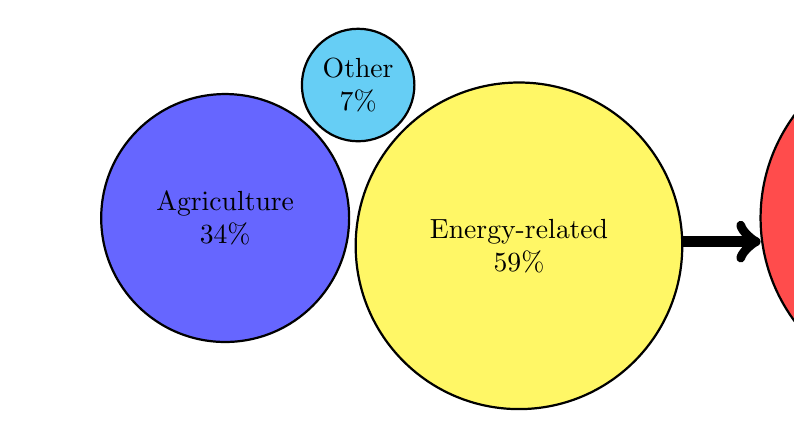
\begin{tikzpicture}[every node/.style={align=center}, pin distance=17mm]
    \pie[cloud,text=inside, radius = 2.7]{34/Agriculture,7/Other,59/Energy-related}
    \draw [->, line width=4pt] (5.8,-0.3) -- (6.8,-.3);
    \hspace{9cm}
    \pie[text=inside,radius=2.2,color={black!30,red!70,yellow!40}]{40/Transport,33/Heat,27/ Electricity}
    \end{tikzpicture}
    \caption{Ireland 2018 GHG Share \cite{Howley2005ENERGY-RELATEDIreland}}
    \label{fig:Ireland2018GHG}
\end{figure}

 While the national GHG should reduce 51\% by 2030, the residential sector is expected to be reduce GHGs even further, due to the higher cost-effectiveness when compared with other sectors. The high ambition in residential is due to its dependency on receiving low carbon intensity electricity. The decarbonisation of the power generation sector is well underway, with carbon intensity falling annually to 375 gCO2/kWh in 2018, 40\% lower than 2005 levels \cite{Howley2005ENERGY-RELATEDIreland}. However the on-shore wind energy capacity is almost saturated, and policy looks to guide investment into off-shore wind to continue a reduction in carbon intensity. Under CAP2019 this continued growth and decarbonisation of the electricity will be the fundamental to lowering energy-related GHG in not only electricity, but heat and transport also. 
 
\begin{figure}[!htbp]
 \centering
 \includegraphics[scale=1.0]{Figures/CAP2019MACC.png} 
 \caption{Climate Action Plan 2019 - Marginal Abatement Cost Curve}
 \label{fig:CAP2019:MACC} \cite{DepartmentofCommunicationsClimateActionandEnvironment2019Climate2019}
\end{figure}

\par
The CAP2019 had a Marginal Abatement Cost Curve (MACC) is based on  based on Environmental Protection Agency (EPA) GHG emission projection report \cite{EPA2018EPAReport} and provides a solid analytical foundation on the most cost-effective pathway to reduce Non-ETS GHG by 30\% in 2030 compared to 2005 levels. The MACC explores technological, behavioural and fuel switching. The x-axis (width of each bar chart) shows the potential reduction of annual MtCO2eq. emissions in 2030 from the technology or fuel switch. The y-axis (height of each bar chart ) shows the associated average cost of abating one tonne of CO2eq. over the 2021 to 2030 period. The columns are organised from the most economical (left side) to the most expensive technology (right side) in EUR/tCO2eq \cite{DepartmentofCommunicationsClimateActionandEnvironment2019Climate2019}. In the least-cost pathway Ireland would increase Onshore wind by 8.2 GW and Offshore would grow to 3.5 GW,this would be expected to save 7 to 8 MtCO2eq. This would help to indirectly reduce the GHG in the residential sector. However specific residential solutions in the MACC include: 
\begin{itemize}
    \item{Retrofit oil boiler existing dwellings to B2 equivalent}
    \item{Switch from oil boilers to heat pumps in existing dwellings}
    \item{Retrofit gas boiler and solid fuel stove existing dwellings to B2 equivalent}
    \item{Introduce CO2-free heating in new buildings}
\end{itemize} 

McKinsey and Company's modelling tools have helped develop the MACC shown in Fig.\ref{fig:CAP2019:MACC}, with more ambitious Non-ETS 2030 target due this year and a national GHG target for 2030, there is a requirement for a new MACC, from which a new residential five-year carbon budgets will arise. 
Sustainable Energy Authority of Ireland (SEAI) and others have been part of the renovation wave in Ireland, the uptake of heat pumps in existing homes is gradually building due to grants, awareness and increasing the ease of upgrades for homeowners, while new homes have a strict regulation to comply with, so heat pumps despite their high capital costs are preferred. The building regulations in 2021 will require a 70\% reduction of CO2 emissions in new dwellings compared to 2005 \cite{DepartmentofHousingGov.ieBuildings}. The CAP2019 plan to deliever a new retrofitting model to upgrade 500,000 existing homes to a Building Energy Rating (BER) ‘B2’ by 2030, highlighting the energy efficiency first approach in how Ireland aims to progress.
 
\subsection{Ireland: Residential Sector Background}
\label{Intro:IreRSDBack}
Among European Union (EU) member states, Ireland has the lowest renewable heat of 6.3\% \cite{Eurostat2021ShareSourcesnrg_ind_ren}.
\par
Ireland’s decarbonisation pathway, is further separated from other EU member states when focusing on the residential sector, this is largely down to Ireland’s high reliance on fossil fuels and settlement patterns of low thermal efficiency of the housing stock. Ireland's lower than average urbanisation which is connected to only 5.8\% of the population of Ireland living in apartments in 2018, the lowest and well below the average EU-27 of 25.3\% \cite{EurostatDistributionSurveyilc_lvho01}, the lower density relates translates to more expensive mitigation. 33\% of the population of the EU were deemed to live in dwellings too large for their needs in 2018, in Ireland the rate was 71.4\% \cite{EurostatShareSurveyilc_lvho50a}.  
Ireland set out national policy objectives under 10 strategic investment priorities \cite{Ireland2018ProjectFramework}. The first of strategic investment priority is ``Compact Growth" which aims to  achieve \textit{``effective density and consolidation, rather than more sprawl of urban development, is a top priority".}, which will indirectly effect both electricity and transport GHG emission. 
In the last 30 years, the extraction of indigenous peat has declined and consequently peat consumption has halved in the last 30 years, and in 2018 peat accounted for 12.3\% of residential GHG emissions. Residential coal GHG emissions has also declined to 6.9\% in 2018. However, the decline in peat and coal has been offset by more significant growth in oil boilers in rural dwellings in the same period, where oil accounts for 34.8\% of residential GHG emissions \cite{Howley2005ENERGY-RELATEDIreland}. Urban dwellings prefer gas as a heating fuel, which is cheaper, more secure ( 61\% of gas in 2018 was indigenous ) and less carbon intensive. Gas accounted for 15.5\% of residential GHG emission in 2018, significantly lower than oil due to the lower carbon intensity. 
Gas Network Ireland (GNI) anticipates that by 2026 or 2027 the supply from Corrib ( Irelands only indigenous gas supply ) will be less than 30\% of 2018 levels \cite{OCleirigh2020ENERGYReport}
In summary, the residential sector is highly reliant on fossil fuels as shown in Fig.\ref{fig:ResFuel}. 

\begin{figure}[!htbp]
 \centering
 \includegraphics[scale=0.5]{Figures/ResidentialFuelUsage.png}
 \caption{Historical Residential Fuel Consumption}
 \label{fig:ResFuel}
\end{figure}
% NOTE THE Y-AXIS IS NOT CORRECT - DATA FROM SEAI ENERGY DATA PORTAL 

Historical fuel usage in one part of understanding residential energy, the other main part is understanding the low thermal efficiency of Irelands housing stock. As mentioned in section \ref{Intro:IreRSD}, Irelands new buildings produce 70\% less GHG emissions than building in 2005, but since the 2008 global financial crisis there has been a considerable slowdown in the growth of housing stock. According to Central Statistics Office (CSO) approx. 85\% of residential buildings are 2005 or older. The BER database, which represents half of the dwelling stock highlights the impact the year of construction has on the expected energy consumption, as shown in Fig.\ref{fig:BERAge}.The BERs are categorised into BER labels, with A1 representing the lowest energy consumption ($\leq 74 kWh/m^2/year$) and G representing the highest energy consumption ($ >450 kWh/m^2/year$) . 


\begin{figure}[!htbp]
 \centering
 \includegraphics[scale=0.4]{Figures/BERAge.png}
 \caption{Building Energy Rating by Age}
 \label{fig:BERAge}
\end{figure}

The poor BERs consequently translates to higher energy bills to maintain comfortable temperature, but in reality it relates to low internal temperatures, which likely results in higher excessive winter mortality \cite{Clinch2000HousingMortality}.The BERs which come from the Energy Performance of Buildings Directive 2002/91/ EC, helps to better understand the housing stock. The BERs are required for new houses, rented houses, sold houses and renovated houses. However, BERs do not take account of actual usage, i.e occupancy behaviour or occupancy density, nor does it take account of the size of the dwelling. The BER labels do therefore leave a gap between actual consumption and expected consumption, I will explain how I approached this problem in the Literature review. 

Fuel Poverty is when a household spends \textit{``10\% or more of income to achieve adequate warmth"}, an element energy reported 28\% of Irish households were in fuel poverty in 2015  \cite{ElementEnergy2015Bottom-upIreland}. While income supports and the \textit{Fuel Allowance and the Household Benefits} provides support to low income households to allievate some the fuel poverty. These payments have been increased over time with a further increase made in Budget 2020, coinciding with the increase in the carbon tax \cite{,EuropeanUnion2020EUObservatory}. As Kerr points out the link between energy and social welfare policy is made explicitly \cite{,EuropeanUnion2020EUObservatory,Kerr2019PoliticsFrance} and O’Meara highlights the health issues associated with Fuel Poverty, which include increased risk of catastrophic cardiovascular or cerebrovascular events \cite{OMeara2016AIreland}. Ironically, this places low income households deeply dependent on fossil fuels for health.



\subsection{Residential Energy Services}
\label{Intro:EnergyServices}

Space heating accounted for the majority of final energy, Fig. \ref{fig:Ireland2018ServiceDemands} shows a snapshot of the residential energy services demands in 2018. As households become more thermal efficient and use higher efficient heating, space heating energy would be expected to decline. The new A-rated dwellings will use less energy for space heating, but Pumps \& Fans energy will increase as mechanical ventilation is used over natural ventilation. 

\begin{figure}[!htbp]
\centering
    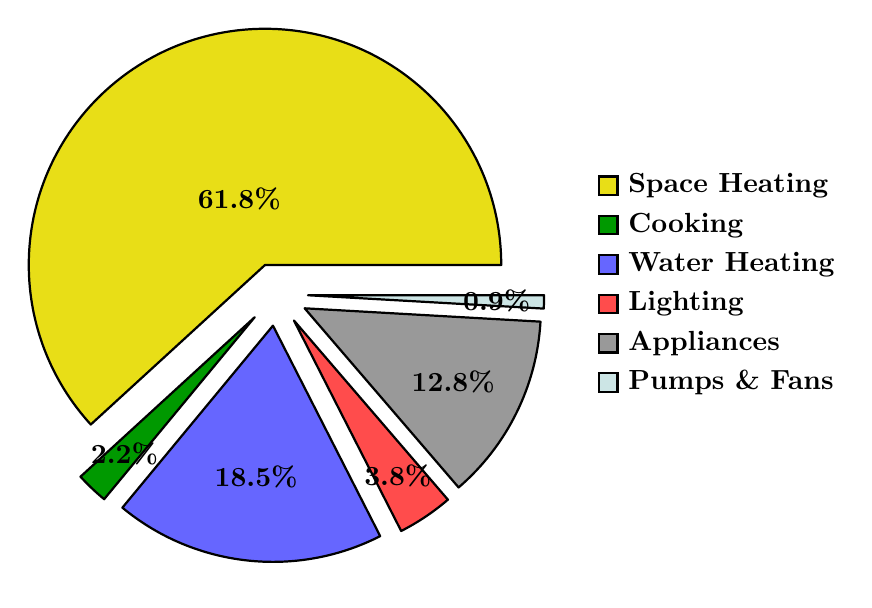
\begin{tikzpicture}
    \tikzstyle{every node}=[font={\bf}]
    \pie[   color = { yellow!90!black, green!60!black, blue!60,
        red!70,
        gray!80,
        teal!20
    }, explode = 0.4, text=legend, radius=3]{61.8/Space Heating, 2.2/Cooking, 18.5/Water Heating, 3.8/Lighting, 12.8/Appliances,0.9/Pumps \& Fans}
    \end{tikzpicture}
    \caption{Ireland 2018 Energy Service Demands}
    \label{fig:Ireland2018ServiceDemands}
\end{figure}

Space heating is therefore central to residential energy policy, other important service energy demands are shown in Fig.\ref{fig:Ireland2018ServiceDemands}. Notably space cooling is absent for the pie chart, but space cooling is accounted for in appliances. The Policy Oriented Tool for Energy and Climate Change Impact Assessment (POTEnCIA) project disaggregated Ireland's residential space cooling from appliances and have output space cooling energy consumption data, shown in Fig.\ref{fig:Cooling} a significant amount of space cooling energy is expected in the Ireland residential sector. 


\begin{figure}[h]
\centering
\begin{tikzpicture}
\begin{axis}[
    x tick label style={
		/pgf/number format/1000 sep=},xlabel={Year},
	y tick label style={
	    /pgf/number},
		ylabel={Energy Consumption($ktoe$)},
		 scaled y ticks = false,
    xmin=2000, xmax=2050,
    ymin=0, ymax=40,
    xtick={2000,2010,2020,2030,2040,2050},
    ytick={0,10,20,30,40},
    ymajorgrids=true,
]
\addplot[
    color=blue,
    mark=square,
    ]
    coordinates {
    (2000,0.6)(2010,3.1)(2020,8.4)(2030,16.3)(2040,26.1)(2050,37)
    };
\end{axis}
\end{tikzpicture}
    \caption{Space Cooling Residential Energy Consumption (Source: POTEnCIA) }
    \label{fig:Cooling}
\end{figure}

The SEAI residential energy report \cite{SustainableEnergyAuthorityofIreland2018EnergySector} provides high resolution detail on energy demands in the residential sector. Variables such as disposable income, appliance ownership, dwelling location, type of occupier status (owner/rented ), BER label and age of dwelling. 

\subsection{Current Energy Policy}
\label{Intro:Policy}
The 2019 Climate Action Plan identified 29 actions that would reduce emissions from the sector by 40-45%.  These actions included:
Reducing fossil fuel use in the sector and moving to electricity to provide heating and hot water in buildings
500,000 building retrofits to a BER B2 / cost optimal equivalent or carbon equivalent
Installation of 600,000 heat pumps, with 400,000 of these in existing buildings
Development of district heating, including two initiatives of municipal scale with the potential to provide heat equivalent to the needs of about 50,000 homes
Complete the rollout of the Support Scheme for Renewable Heat
Increasing the number of Sustainable Energy Communities to 1,500

\subsubsection{Electricity}
\par
Decarbonising Electricity is key for Ireland, both the \textit{``stick"} (tax) approach which aims to deter investment in fossil fuel power generation, and the \textit{``carrot"} (subsidies) approach which aims to encourage renewable electricity is applied in Irish policy.
In Ireland, a €15/tCO2 carbon tax was introduced in 2009 to influence fossil fuel demand. The carbon tax receipts grew every year from 2010 to 2018 \cite{AnOffice}. Ireland's current carbon tax of €33.50/tCO2 will rise to €100/tCO2 in 2030. Many countries have taken this approach, especially in Europe, where Finland was the first country to introduce a carbon tax in 1990, while Sweden were second to introduce a carbon tax after Finland, the carbon tax rate is the highest in the world at €108.81/tCO2. A carbon price or tax now accounts for approx. 15\% of GHG emissions \cite{WorldBankGroup2020State2020}. 
The Renewable Energy Feed-in Tariff (REFIT) schemes were designed to incentives investment in renewable electricity to achieve legally binding renewable targets under 2009/28/EC. REFIT operates  by  guaranteeing  new renewable generation and biomass a minimum price for electricity over a 15 year period. The last REFIT schemes closed in December 2015. In 2020 REFIT was replaced by the Renewable Electricity Support Scheme (RESS), which supports to renewable electricity projects to help Ireland achieve 2030 climate targets, especially the 70\% renewable electricity target. RESS delivers for communities to participate in renewable energy projects and increasing technology diversity by broadening the renewable electricity technology mix, where almost 800 MW of solar has been approved in RESS-1 \cite{Eirgrid2020RenewableResults}, this builds alot on the current solar capacity of 16 MW, while making significant progress towards the CAP2019 target of 1500 MW by 2030.

\subsubsection{Heat}
Domestic supports for renewable heat or energy efficiency is through SEAI grants,\begin{itemize}
    \item {Insulation}
    \subitem {Attic}
    \subitem {Cavity Wall}
    \subitem {Internal - Dry Lining}
    \subitem {External}
    \item {Heat Pumps}
    \subitem {Air to Water}
    \subitem {Ground Source to Water}
    \subitem {Exhaust Air to Water}
    \subitem {Water to Water}
    \subitem {Air to Air}
    \item {Heating Controls}
    \item {Solar Water Heating}
\end{itemize}

This report is a study of potential design options for a Renewable Heat Incentive (RHI) f

-  critical for the development of renewable gas projects in Ireland.European Commission’s decision on State aid for the Support Scheme for Renewable Heat (SA.50807).
GNI Vision 2050 - 20\% renewable gas by 2030
While the electricity network reaches all residential dwellings, The gas network reaches 40\% or 680,000 dwellings in towns and cities. The 2030 gas decarbonisation targets, set by GNI  
and  with biomethance and renewable gas targets for 2030, X\%. The district heating networks are new and currently only two in Dublin which reach about XX houses, 2030 target X%. large amount of data centres. Other future heating fuel options such as hydrogen, HVO, solar may also play a part. 
Gas Networks Ireland (GNI) has a strategic plan to achieve 20% Renewable Gas on the network by 2030 
Further investigate decarbonisation options such as hydrogen vehicles, biomethane and AD
substitutes for natural gas - See \ref{fig:CAP2019:MACC} shows biomethane as the most expensive options..

\subsection{TIMES Ireland Model (TIM)}
\label{Intro:TIM}
\par
TIM was built to help Ireland provide a pathway to achieve 2030 and 2050 targets. The residential sector plays a key part of this and it was built from the SEAI 2018 energy balance, the BER database and CSO data. The data filtration process used in the residential sector, derived a lot of conversation of the BER database, a group know as Ireland Energy Wiki by the National Retrofitting Modelling Group grew from building the residential sector, questions about the filters, default values, assumptions around thermal equations (EC..) and uncertainties were used to improve the data before it was used in TIM . TIM has many internal project deadines, which required extensive meetings about the data, constraints and results as the modelling was progressing. The data and results were presented to 30 external reviewers to provide feedback, this process proved invaluable having different expertise with different presepectives enabled TIM to fill in gaps. TIM will also be open platform to help improve the model and provide transparency. TIM’s residential sector was built in parallel with LEAP’s residential sector, so that residential sector can easily simulate policy. The demand for results from TIM has increased significantly with increased government ambition, TIM will provide input into CAP 2021 and Ireland’s carbon budgets, working with DECC and the CCAC respectively will also provide feedback and improve the robustness of TIM. for these reasons TIM residential sector is a state of the art modelling platform. 
%GRAPH OF IRELAND DECARBONISATION TARGETS  VS OTHER COUNTRIES - DIFFERENT INTRASTATE and RESOURCE AT BIDENS ENERGY SUBMIT - DENMAKR TOP 2018, 
	ESOM can be used to start the conversation on..
Look at other ESOM, brief explain…
Other residential sectors..
CAP2019 - Choosing the Pathways which Create the Least Burden
and Offer the Most Opportunity for Ireland
\section{Literature Review}
\label{LitR}
``How should Ireland set GHG targets in the residential sector?” 
 % LIT REW INPUT DATA - EU \cite{Simoes2013TheProject} 

%the new A-rated houses behave distinctively different which much less demand on space heating and with pumps and fans energy consumption usage increasing, while appliance end use is increasing across the BER ratings. The number of appliances has increased rapidly and while energy efficient improves are  reducing the energy per appliance, it is overshadowed by the growth in electrical appliances. There retrofitting grant which  requires building to have a HLI indication of 2 or less before a heat pump grant can be installs. Ireland’s aim of retrofitting 0.5 million homes from the existing 1.7 million in the before 2030. The effect of these targets also stretches out across the construction sector. The savings from retrofits will decrease fossil fuel energy usage, while most houses 00\% would need to get heat pumps too, to fulfil 0.4 million existing houses getting heat pumps.  This energy efficiency first approach would allow for future technology choices, when current boiler are not at end of life. 

%Lorem ipsum dolor sit amet, consectetur adipiscing \citep{Fabioetal2013} elit, sed do eiusmod tempor incididunt ut labore et dolore magna aliqua. Ut enim ad minim veniam, quis nostrud \citet{Blondeletal2008} exercitation ullamco laboris nisi ut aliquip ex ea commodo consequat. Duis aute irure dolor in reprehenderit in voluptate velit esse cillum dolore eu fugiat nulla pariatur. Excepteur sint occaecat cupidatat non proident, sunt in culpa qui officia deserunt mollit \citep{Blondeletal2008,FabricioLiang2013} anim id est laborum.

%Lorem ipsum dolor sit amet, consectetur adipiscing elit, sed do eiusmod tempor incididunt ut labore et dolore magna aliqua. Ut enim ad minim veniam, quis nostrud exercitation ullamco laboris nisi ut aliquip ex ea commodo consequat. Duis aute irure dolor in reprehenderit in voluptate velit esse cillum dolore eu fugiat nulla pariatur. Excepteur sint occaecat cupidatat non proident, sunt in culpa qui officia deserunt mollit anim id est laborum see appendix~\ref{sec:sample:appendix}.

%% The Appendices part is started with the command \appendix;
%% appendix sections are then done as normal sections
\section{Acknowledgements}
\label{sec:Acknowledgements}
%CAPACITY is funded under the Climate Action Modelling Group (CAMG) by DECC
% https://www.marei.ie/project/capacity/
CHIMERA is supported by a research grant from Science Foundation Ireland (SFI) and the National Natural Science Foundation of China (NSFC) under the SFI-NSFC Partnership Programme, grant no. 17/NSFC/5181 and
supported by MaREI, the SFI Research Centre for Energy, Climate, and Marine [Grant No: 12/RC/2302\_P2]


https://www.marei.ie/project/chimera/
\appendix

\section{Sample Appendix Section}
\label{sec:sample:appendix}
Lorem ipsum dolor sit amet, consectetur adipiscing elit, sed do eiusmod tempor section \ref{sec:Introduction} incididunt ut labore et dolore magna aliqua. Ut enim ad minim veniam, quis nostrud exercitation ullamco laboris nisi ut aliquip ex ea commodo consequat. Duis aute irure dolor in reprehenderit in voluptate velit esse cillum dolore eu fugiat nulla pariatur. Excepteur sint occaecat cupidatat non proident, sunt in culpa qui officia deserunt mollit anim id est laborum.

%% If you have bibdatabase file and want bibtex to generate the
%% bibitems, please use
%%

\printbibliography

%% else use the following coding to input the bibitems directly in the
%% TeX file.

%%\begin{thebibliography}{00}


% %% \bibitem[Author(year)]{label}
% %% Text of bibliographic item

% \bibitem[ ()]{}

% \end{thebibliography}
\end{document}
\endinput
%%
%% End of file `elsarticle-template-harv.tex'.
